\documentclass[../main]{subfiles}

%TeXromancers series page template
%by derivada.schwarziana

\begin{document}

%please update these for each book release:

\newcommand{\bookauthor}{J. W. Milnor and J. D. Stasheff}
\newcommand{\shortbookauthor}{Milnor and Stasheff}
\newcommand{\booktitle}{Characteristic Classes}
\newcommand{\booksubtitle}{}

\newcommand{\bookcoverTeXromancers}{Revised and modernized edition by}

\newcommand{\bookcoverpicture}{
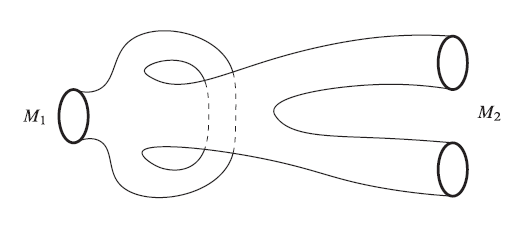
\includegraphics[height=21em]{./fig6.PNG}
}

\newcommand{\bookoriginaledition}{1965}
\newcommand{\bookthisedition}{2022}

%these are meant for the back cover
%both should have ~100 words
\newcommand{\bookreview} 
{The theory of characteristic classes provides a meeting ground for the various disciplines of differential topology, differential and algebraic geometry, cohomology, and fiber bundle theory. As such, it is a fundamental and an essential tool in the study of differentiable manifolds.
\\[1em]

In this volume, the authors provide a thorough introduction to characteristic classes, with detailed studies of Stiefel-Whitney classes, Chern classes, Pontrjagin classes, and the Euler class. Three appendices cover the basics of cohomology theory and the differential forms approach to characteristic classes, and provide an account of Bernoulli numbers.
\\[1em]

Based on lecture notes of John Milnor, which first appeared at Princeton University in 1957 and have been widely studied by graduate students of topology ever since.
}

\newcommand{\bookauthorbio}
{Awards and Recognition
\\[1em]

\defemph{John Milnor}, Winner of the 2011 Abel Prize from the Norwegian Academy of Science and Letters
\\[1em] Winner of the 2011 Leroy P. Steele Prize for Lifetime Achievement, American Mathematical Society
}
\newcommand{\authorbiosource}{Princeton press}     %BOOK INFO GOES HERE -- please update _BOOKINFO.tex for new books
%http://paletton.com/#uid=b14333r0kkAw01RZWclMishq8B4eb

\definecolor{tyellow}{HTML}{FFD05B}
\definecolor{tyellowlight}{HTML}{FFE39D}
\definecolor{tyellowlighter}{HTML}{FFFBF0}
\definecolor{tyellowdark}{HTML}{D09B18}
\definecolor{tyellowdarker}{HTML}{715000}

\definecolor{tturq}{HTML}{3EAF7F}
\definecolor{tturqlight}{HTML}{86DAB6}
\definecolor{tturqlighter}{HTML}{EEFCF6}
\definecolor{tturqdark}{HTML}{118F59}
\definecolor{tturqdarker}{HTML}{004D2C}

\definecolor{tblue}{HTML}{3E83A1}
\definecolor{tbluelight}{HTML}{86BCD4}
\definecolor{tbluelighter}{HTML}{EEF8FC}
\definecolor{tbluedark}{HTML}{156283}
\definecolor{tbluedarker}{HTML}{033247} %colors

%book series page
\newpage
\thispagestyle{empty}

\begin{center}
    \Huge{
    
\includegraphics[height=1.5em]{texromancers_gray.pdf}
    \raisebox{0.55em}{\TeX{}romancers}
    }
    
    \normalsize{A collaborative typesetting project}
\end{center}

\noindent\makebox[\linewidth]{\rule{\linewidth}{0.4pt}}

\bigskip

This book is the product of a community effort. It was typeset by \TeX{}romancers: an enthusiast group of mathematicians (for the most part), consisting of people organized on Discord. The reader should contact \texttt{amanzoo1@asu.edu} if they are interested in joining the group. Link to the group's page: \url{https://aareyanmanzoor.github.io/Texromancers.html}.

\noindent\makebox[\linewidth]{\rule{\linewidth}{0.4pt}}

\bigskip

\noindent\textbf{More books in this series:}
\begin{itemize}
    \item J. F \textsc{Adams}, \textbf{Stable Homotopy and Generalised Homology}
        \begin{itemize}
            \item Available at \url{https://people.math.rochester.edu/faculty/doug/otherpapers/Adams-SHGH-latex.pdf}
        \end{itemize}
    \item Noel J. \textsc{Hicks}, \textbf{Notes on Differential Geometry}
        \begin{itemize}
            \item Available at \url{https://aareyanmanzoor.github.io/assets/hicks.pdf}
        \end{itemize}
    \item Hideyuki \textsc{Matsumura}, \textbf{Commutative Algebra}
        \begin{itemize}
            \item \url{https://aareyanmanzoor.github.io/assets/matsumura-CA.pdf}
        \end{itemize}
    \item John Milnor and James Stasheff, \textbf{Characteristic Classes}
    \begin{itemize}
        \item Available at \url{https://aareyanmanzoor.github.io/assets/books/characteristic-classes.pdf}
    \end{itemize}
\end{itemize}

\vfill



\end{document}
